\documentclass[a4paper,12pt]{article}
% ======================== Einstellungen ========================
\usepackage[utf8]{inputenc}
\usepackage[T1]{fontenc}
\usepackage[ngerman]{babel}
\usepackage{caption}
\captionsetup[table]{labelfont=bf,textfont=it}
\usepackage{geometry}
\usepackage{graphicx}
\usepackage{tabularx}
\usepackage{booktabs}
\usepackage{listings}
\usepackage{xcolor}
\usepackage{float}
\usepackage{amsmath}
\usepackage{titlesec}
\usepackage{enumitem}
\usepackage{multicol}
\usepackage{multirow}
\usepackage{makecell}
\usepackage{xcolor}
\usepackage[pdfencoding=auto]{hyperref}
\usepackage{textcomp}
\usepackage{tocloft}
\renewcommand{\cftsecleader}{\cftdotfill{\cftdotsep}}
\renewcommand{\cftsubsecleader}{\cftdotfill{\cftdotsep}}
\renewcommand{\cftsubsubsecleader}{\cftdotfill{\cftdotsep}}
\newcommand{\pfeil}{$\rightarrow$}
\usepackage[pdfencoding=auto]{hyperref}
\hypersetup{
    colorlinks=true,
    linkcolor=blue,
    filecolor=magenta,      
    urlcolor=cyan,
    pdftitle={Einführungsprojekt für Informatiker},
    pdfauthor={864154},
    pdfsubject={Pong-Spielentwicklung},
    pdfkeywords={Python, PyGame, OOP}}
\titleformat{\section}
{\normalfont\Large\bfseries}{\thesection}{1em}{}
\titleformat{\subsection}
{\normalfont\large\bfseries}{\thesubsection}{1em}{}
\titleformat{\subsubsection}
{\normalfont\normalsize\bfseries}{\thesubsubsection}{1em}{}
\geometry{a4paper, left=25mm, right=25mm, top=25mm, bottom=25mm}
\lstset{
    basicstyle=\ttfamily\small,
    keywordstyle=\color{blue},
    commentstyle=\color{gray},
    stringstyle=\color{red},
    frame=single,
    breaklines=true,
    postbreak=\mbox{\textcolor{red}{$\hookrightarrow$}\space},}
\begin{document}
% ======================== Deckblatt ========================
\begin{titlepage}
    \centering
    \vspace*{2cm}
    {\Huge\bfseries Mücahid Emin Tomakin}\\[0.5cm]
    {\Huge\bfseries 864154}\\[0.5cm]
    \vfill
    {\LARGE B-INF01XX - Einführungsprojekt für Informatiker}\\[0.3cm]
    {\large Pong-Spielentwicklung}\\[0.1cm]
    {\large Aufgaben 1–4}\\[1cm]
    {\large Herr Marion Lammarsch, Dozent}\\[0.2cm]
    {\large Frau Joachim Lammarsch, Dozentin}\\[2cm]
    {\large 20.11.2024 – 21.11.2024}\\[0.2cm]
    {\large 16:00 – 20:00 Uhr}\\[2cm]
    \vfill
    \vspace*{1cm}
\end{titlepage}
\clearpage
% ======================== Inhalts-, Abbildungs, Tabellen- und Codeverzeichnis ========================
\renewcommand{\contentsname}{Inhaltsverzeichnis}
\tableofcontents
\clearpage
\listoffigures
\addcontentsline{toc}{section}{Abbildungsverzeichnis}
\clearpage
\listoftables
\addcontentsline{toc}{section}{Tabellenverzeichnis}
\clearpage
\renewcommand{\lstlistlistingname}{Codeverzeichnis}
\lstlistoflistings
\addcontentsline{toc}{section}{Codeverzeichnis}
\clearpage
% ======================== Einführung ========================
\section{Einführung}
Das Projekt heißt \textbf{B-INF01XX – Einführungsprojekt für Informatiker}.
In diesem Projekt geht es um einen Arbeitsauftrag zwischen dem Kunden, dem Manager und dem Entwickler so wie es in der Arbeitswelt vorkommen könnte zu Simulieren. Dabei nehmen die Studierende die Rolle des IT-Manager und des IT-Entwicklers und die Lehrenden (Expertengeführte Projektbefgleiter) die Rolle des Kunden entgegen.
Anfangs wurden mittels einer Virtuellen Maschine die von den Projektbefgleitern zu Verfügung gestellten Betriebssystems aufgesetzt, theoretisches Wissen gelehrt, mehrere kleinere Aufgaben, sowie Hausaufgaben erledigt, welche auf das tatsächliche Projekt \textbf{Pong} aufbauen sollten. Daher werden diese bei der Dokumentation nicht miteinbezogen.
Da der Adressat des Projektdokumentations ein erfahrener Softwarearchitekt ist wird ausschließlich der Ablauf des Projekts erläutert und nicht auf die Fachbegriffe und auf die Verwendung der Programmiersprache eingegangen.
\clearpage
% ======================== Einzelne Kriterien des Projektes ========================
\section{Einzelne Kriterien des Projektes}
\begin{center}
    \begin{tabular}{|l|l|l|l|}
        \hline
        Zeit & Qualität & Quantität & Kosten \\
        \hline
    \end{tabular}
\end{center}
\subsection{Zeit}
Der gesamte Zeitaufwand des Projektes Pong beträgt 225 Minuten \textit{(3,75 Stunden)}. Die einzelnen Teile der Projektlaufzeit sind mittels der Tabelle aufgelistet.
\begin{table}[ht]
\centering
    \begin{tabular}{|l|l|}
        \hline
        \textbf{Einzelne Teilschritt} & \textbf{Teilprojektlaufzeit in Minuten} \\
        \hline
        Kickoff Meeting & 20 \\
        Storyboard & 30 \\
        Verbale Beschreibung der Aufgabenstellung & 20 \\
        Nominal- und Verbalphrasenanalyse & 60 \\
        CRC-Karte & 70 \\
        Review & 0 \textit{aufgrund Expertengeführte Projektbefgleitung} \\
        Konzept- und Implementierungsdiagramm & 0 \textit{aufgrund Expertengeführte Projektbefgleitung} \\
        Implementierung & 25 \\
        Testraum & 5 \\
        Projektabschluss & 0 \textit{aufgrund Expertengeführte Projektbefgleitung} \\
        \hline
    \end{tabular}
    \caption{Der gesamte Zeitaufwand}
\label{tab:der-gesamte-zeitaufwand}
\end{table}
\subsection{Qualität}
Alle angeforderten Funktionalitäten wurden erfüllt \textit{(Spielfeld, Spielerschläger, Computerschläger, Ball, Punkteanzeige)}, die Nutzbarkeit ist einfach gestrickt \textit{(Betätigung einer beliebigen Taste zum Spielstart und Maussteuerung)} uns sehr schnell zu erlernen und Wartbarkeit ist mittels der Bibliotheken \textit{(Py Game und Spiel)} auf das Minimum gesetzt und somit relativ simple.
\subsection{Quantität}
Die Anzahl der ausgelieferten Funktionen ist nicht sehr hoch und somit als nicht sehr anspruchsvoll zu definieren.
\subsection{Kosten}
Die Gesamtkosten hängen abgesehen von den geringen bis in diesem Fall kaum vorhandenen Ausgaben für Equipment \textit{(PC)}, Lizenzen zur Nutzung von Software \textit{(Python + Bibliotheken)} und die Erstellung der Storyline maßgeblich von den Personalkosten ab. \par\vspace{0.5em} Auch das Zielsystem iOS, Android, iPadOS, watchOS, Linux, MacOS oder Windows ist wichtig. Dieses Projekt wurde ausschließlich für das Linux Betriebssystems entwickelt.
\clearpage
% ======================== Projektauftrag ========================
\section{Projektauftrag}
\subsection{Kickoff-Meeting}
Bei einem Kickoff Meeting kommen alle Beteiligten zusammen, um das Projekt zu starten. Es legt den Grundstein für den weiteren Verlauf und dient dazu, alle Beteiligten auf denselben Wissensstand zu bringen. Das Meeting ist besonders wichtig, um Missverständnisse zu vermeiden und einen gemeinsamen Fokus auf die Projektziele zu setzen. Dabei ist es als Entwickler essentiell möglichst viele Fragen zu stellen und alle Fragezeichen aus dem Kopf zu bekommen. Manchmal denkt man sich die Frage die mir durch den Kopf geht ist eigentlich nicht so wichtig und unlogisch, jedoch kann es vorkommen, dass genau diese unwichtige Frage eine andere noch zu diesem Zeitpunkt ungeklärte und später zu Komplikationen führende Frage eines anderen triggert und man dem Kunden dadurch eine Sicht zu zeigen vermag, den der Kunde selber nicht berücksichtigt hatte. Dem Kunden ist dies genauso wichtig, da dieser möglicherweise nicht ganz in der Materie ist und merkt, dass dieser nicht wirklich weiß was er wirklich haben möchte bzw. wie genau. \par\vspace{0.5em} Zunächst wurde das Projekt präsentiert. Damit die Projektziele und der Umfang, warum das Projekt wichtig ist, die erwarteten Ergebnisse, Rollen Verteilung und Klärung der Verantwortlichkeiten, Überblick über den Arbeitsablauf, Klärung von Zweifeln oder Missverständnissen und am Ende Offene Fragen und Feedback von den Teilnehmern.
\subsubsection{Einige Fragen haben folgendermaßen ausgesehen:}
\begin{itemize}
    \item Soll das Spiel Cross-Plattform kompatibel sein? \\
    \textit{Das Zielsystem ist ein Laptop/Desktop Gerät. Daher alle drei gängigen Betriebssysteme, darunter Linux, Windows und MacOS.}
    \item Wie soll sich der Ball bei einem Abprall verhalten? \\
    \textit{Der Ball soll im Einfalles- und Ausfallswinkel Abprallen.}
    \item Hat das Spiel ein Ende? \\
    \textit{Nein, die Punkte sollen bei einem Fehlschlag einfach auf 0 gesetzt und in einer Endlosschleife weitergehen, bis man das Spiel selber mit einem Klick auf das „x" an der oberen Ecke beendet.}
\end{itemize}
Der Auftrag besteht im Grunde darin ein Spiel-Projekt mittels Python unter Verwendung der Bibliotheken Py Game und Spiel zu entwickeln. Dabei geht es um ein Spiel namens \textbf{Pong} in dem ein Ball sich über den Bildschirm bewegt und von den Schlägern die sich vertikal am linken und rechten Bildschirmrand bewegen oder den oberen und unteren Bildschirmrändern abprallt. Das Ziel dabei ist es den Ball so zurückschlagen, dass der Gegner ihn nicht erwischt. Ein Punkt wird erzielt, wenn der Ball am Gegner vorbeigeht. Dabei ist der Gegner \textit{(rechter Schläger)} ein Computer der sich parallel zum Ball bewegt und somit unschlagbar ist. Die Steuerung \textit{(linker Schläger/Spieler Schläger)} soll mit durch verschieben der Maus erfolgen, um den Schläger nach oben oder unten zu bewegen.
\clearpage
% ======================== Anforderungsdefinition ========================
\section{Anforderungsdefinition}
\subsection{StoryBoard}
Mittels eines Storyboards ist es möglich die Handlung und die Szenen eines Spiels visuell darzustellen. Dabei ist die Struktur wie ein Comic oder eine Serie von Bildern aufgebaut. Es hilft dabei, den Ablauf und die Schlüsselmomente zu planen und diese zu visualisieren, bevor die Entwicklung beginnt. \par\vspace{0.5em} Dies hat den Vorteil, dass man eine klare Vision hat. Es bietet eine klare Vorstellung von der Handlung und den Szenen. Desweiterem ist die Kommunikation ein essentielles Schlüsselwort. Erleichtert die Zusammenarbeit im Team, da alle eine gemeinsame Referenz haben. Zu guter Letzt spart dies viel Zeit, da Fehler frühzeitig erkannt und korrigiert werden können, was das spätere Aufwand spart.
\subsubsection{Gemeinsames Storyboard:}
Aus den Endresultaten aller Projektbeteiligten wurde ein gemeinsames Storyboard festgelegt.
\begin{figure}[H]
\begin{minipage}{0.48\textwidth}
    \centering
    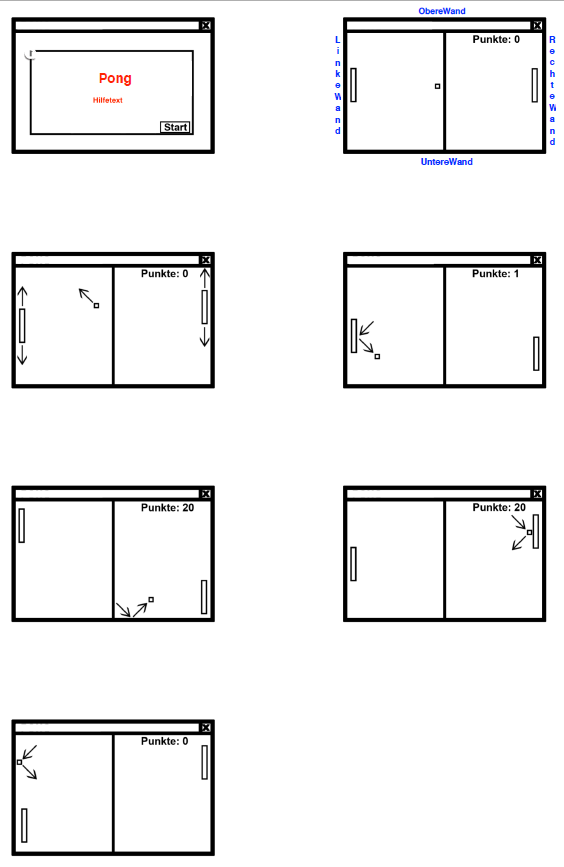
\includegraphics[width=\textwidth]{./img/StoryBoard.png}
    \caption{Gemeinsames StoryBoard}
    \label{fig:gemeinsames-storyboard}
\end{minipage}
\hfill
\begin{minipage}{0.48\textwidth}
    Zu Beginn erschein eine Spielemenu, in dem man im Anschluss zum Spiel startet. \par\vspace{0.3em} Das Spielfeld besteht aus 4 Wänden, 2 Schlägern einem Ball und dem Punktestanzeiger. \par\vspace{0.3em} Die Schläger können sich auf der Y-Achse rauf und runter bewegen wehrend sich der Ball auf der X- und Y-Achse diagonal bewegen kann. \par\vspace{0.3em} Falls der Ball mit dem Schläger in Kontakt kommt wird es dem Winkel entsprächen \textit{(Einfallswinkel und Ausfallswinkel)} abgeprallt. \par\vspace{0.3em} Falls dieser mit der Wand in Kontakt kommt wird dieser ebenfalls dem Winkel entsprechend abgeprallt. \par\vspace{0.3em} Sollte der Spieler auf der linken Seite den Ball schlagen können wird nur dann der Punkteanzeige um 1 erhöht. \par\vspace{0.3em} Sollte dieser dies nicht schaffen und der Ball berührt die linke Wand wird der Punkteanzeige wird auf 0 zurückgesetzt. \par\vspace{0.3em} Bei Kontakt mit allen anderen Wänden wird der Ball nur abgeprallt. \par\vspace{0.3em} Das Spiel hat kein wirkliches „Ende" hat läuft es immer sie weiter bis der Spieler rechts oben auf dem x Button drückt und das Spiel manuell beendet.
\end{minipage}
\end{figure}
\subsubsection{Mein eigenes Storyboard:}
Im Vergleich dazu mein eigenes Storyboard:
\begin{figure}[H]
    \centering
    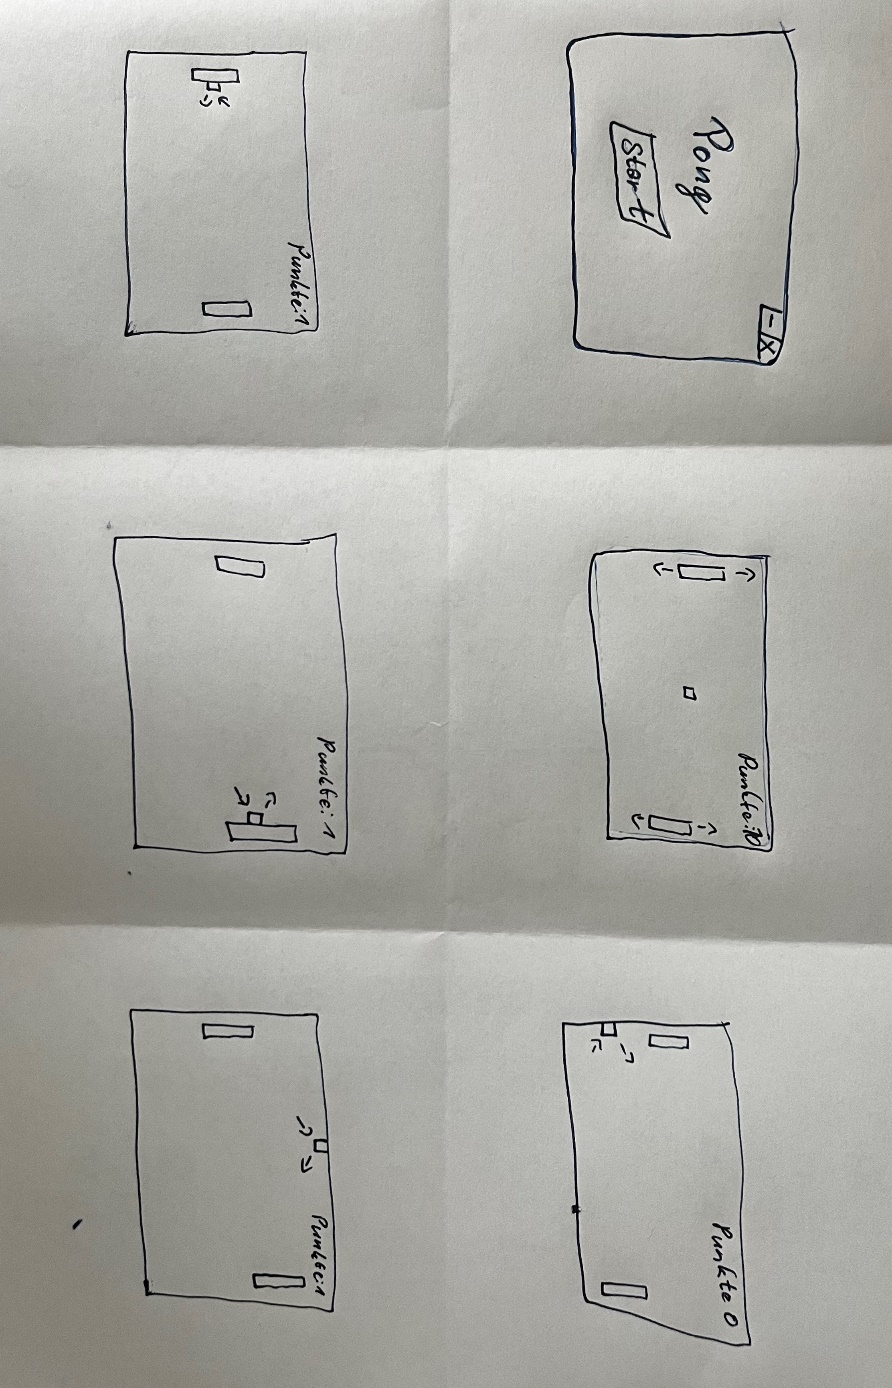
\includegraphics[width=0.6\textwidth,angle=90]{./img/EigenesStoryBoard.jpg}
    \caption{Mein eigenes Storyboard}
    \label{fig:mein-eigenes-storyboard}
\end{figure}
Als erstes fällt bei fasst allen Szenen auf, dass der x Button auf der rechten oberen Seite fehlt. Des weiterem wurden die Wände nicht bezeichnet und es fehlt die Trennlinie in der Mitte. \par\vspace{0.5em} Man kann sehen, dass die Schläger sich nur vertikal rauf und runter bewegen und der Ball bei einer kollabierung sich gemäß Ein- und Ausfallswinkel bewegt.
\subsection{Verbale Beschreibung der Aufgabenstellung}
Das \textcolor{red}{Spiel} \textcolor{blue}{heißt} \textcolor{red}{Pong}. Es \textcolor{blue}{gibt} einen \textcolor{red}{Startbildschirm}. Es \textcolor{blue}{gibt} einen \textcolor{red}{Hilfetext} und einen \textcolor{red}{Startknopf}. Der rechteckige \textcolor{red}{Ball} ist in der \textcolor{red}{Mitte}. Es \textcolor{blue}{gibt} eine \textcolor{red}{Trennlinie} in der \textcolor{red}{Mitte}. Es \textcolor{blue}{gibt} einen \textcolor{red}{Punktestand} oben rechts. Es \textcolor{blue}{gibt} vier \textcolor{red}{Spielfeldbegrenzungen}. Der \textcolor{red}{Spielerschläger} \textcolor{blue}{befindet} sich links und vertikal in der \textcolor{red}{Mitte}. Es \textcolor{blue}{gibt} einen \textcolor{red}{Computerschläger} auf der rechten \textcolor{red}{Seite}. Die \textcolor{red}{Punkte} \textcolor{blue}{starten} bei \textcolor{red}{Null}. Die beiden \textcolor{red}{Schläger} sind rechteckig. Der rechteckige \textcolor{red}{Ball} \textcolor{blue}{bewegt} sich diagonal. Beide \textcolor{red}{Schläger} können sich nur in vertikaler \textcolor{red}{Richtung} \textcolor{blue}{bewegen}. \textcolor{blue}{Trifft} der \textcolor{red}{Spielerschläger} den \textcolor{red}{Ball} \textcolor{blue}{erhöht} sich der \textcolor{red}{Punktestand} um \textcolor{red}{Eins}. Der \textcolor{red}{Ball} \textcolor{blue}{fliegt} mit \textcolor{red}{Einfallswinkel} gleich \textcolor{red}{Ausfallswinkel} weiter. Der \textcolor{red}{Ball} \textcolor{blue}{prallt} mit \textcolor{red}{Einfallswinkel} gleich \textcolor{red}{Ausfallswinkel} von der \textcolor{red}{Wand} oben und unten ab. Der \textcolor{red}{Computerschläger} \textcolor{blue}{orientiert} sich immer an der \textcolor{red}{Höhe} des \textcolor{red}{Balls}. Der \textcolor{red}{Ball} \textcolor{blue}{prallt} mit \textcolor{red}{Einfallswinkel} gleich \textcolor{red}{Ausfallswinkel} vom \textcolor{red}{Computerschläger} ab. Der \textcolor{red}{Ball} \textcolor{blue}{trifft} die \textcolor{red}{Wand} hinter dem \textcolor{red}{Spielerschläger}. Der \textcolor{red}{Punktestand} wird auf \textcolor{red}{Null} \textcolor{blue}{gesetzt}. Der \textcolor{red}{Ball} \textcolor{blue}{fliegt} mit \textcolor{red}{Einfallswinkel} gleich \textcolor{red}{Ausfallswinkel} weiter.
\clearpage
Mittels der verbalen Beschreibung der Aufgabenstellung ist es uns gelungen eine prägnante, textuelle Zusammenfassung der allgemeinen Funktionen und Regeln des Spiels zu verfassen. Sie beschreibt das Gameplay, die Interaktionen, die Logik und die Benutzeroberfläche in einfacher Sprache, ohne auf technische Details einzugehen. Dabei wurden Alle Nomen rot und alle Verben blau markiert um diese später bei Nominal- und Verbalphrasenanalyse zu gebrauchen. \par\vspace{0.5em} Die herausstechenden Vorteile der verbalen Beschreibung der Aufgabenstellung ist zuerst die Klarheit, es Fördert das Verständnis zwischen allen Beteiligten. Daraus folgt die Vermeidung von Missverständnissen. Dieser Stellt sicher, dass alle die gleichen Anforderungen verstehen. Des weiterem auch im späteren Verlauf in der Nominal- und Verbalphrasenanalyse ist dies ein Basis für die Umsetzung und dient als Grundlage für die technische Entwicklung. Zu guter Letzt dient es zu einer Strukturierten Ergebnis.
\clearpage
% ======================== Analyse ========================
\section{Analyse}
\subsection{Nominalphrasenanalyse (Substantiv-Technik)}
\begin{multicols}{3}
\textbf{Spiel}
\begin{itemize}
    \item[\textendash] \emph{Startbildschirm}
    \item[\textendash] \emph{Hilftext}
    \item[\textendash] \emph{Startknopf}
    \item[\textendash] \emph{Pong}
\end{itemize}
\textbf{Ball}
\begin{itemize}
    \item[\textendash] \emph{Richtung}
    \item[\textendash] \emph{Einfallswinkel}
    \item[\textendash] \emph{Ausfallswinkel}
    \item[\textendash] \emph{Höhe}
\end{itemize}
\textbf{Schläger}
\begin{itemize}
    \item[\textendash] \emph{Spielerschläger}
    \item[\textendash] \emph{Computerschläger}
    \item[\textendash] \emph{Richtung}
    \item[\textendash] \emph{Höhe}
\end{itemize}
\end{multicols}
\begin{multicols}{2}
\textbf{Punktestand}
\begin{itemize}
    \item[\textendash] \emph{Null}
    \item[\textendash] \emph{Eins}
\end{itemize}
\textbf{Spielfeldbegrenzung}
\begin{itemize}
    \item[\textendash] \emph{Trennlinie}
    \item[] \phantom{\emph{Eins}}
\end{itemize}
\end{multicols}
\vspace{0.5em}\textbf{Gestrichen:}
\begin{center}
    \begin{tabular}{|l|l|l|l|}
        \hline
        Mitte = Trennlinie & Punkt = Punktestand & Seite = Wand = Spielfeldbegrenzung \\
        \hline
    \end{tabular}
\end{center}
\subsection{Verbalphrasenanalyse}
\begin{multicols}{3}
\textbf{Punktestand}
\begin{itemize}
    \item[\textendash] \emph{befinden()}
    \item[\textendash] \emph{setzen()}
\end{itemize}
\textbf{Schläger}
\begin{itemize}
    \item[\textendash] \emph{befinden()}
    \item[\textendash] \emph{bewegen()}
\end{itemize}
\textbf{Ball}
\begin{itemize}
    \item[\textendash] \emph{bewegen()}
    \item[\textendash] \emph{prallen()}
\end{itemize}
\end{multicols}
\begin{multicols}{3}
\textbf{Hilftext}
\begin{itemize}
    \item[\textendash] \emph{befinden()}
\end{itemize}
\textbf{Startknopf}
\begin{itemize}
    \item[\textendash] \emph{befinden()}
\end{itemize}
\textbf{Spielfeldbegrenzung}
\begin{itemize}
    \item[\textendash] \emph{befinden()}
\end{itemize}
\end{multicols}
\begin{multicols}{2}
\textbf{Spielerschläger \textit{(Schläger)}}
\begin{itemize}
    \item[\textendash] \emph{orientieren() \#durch Spieler}
\end{itemize}
\textbf{Computerschläger \textit{(Schläger)}}
\begin{itemize}
    \item[\textendash] \emph{orientieren() \#anhand des Balls}
\end{itemize}
\end{multicols}
\vspace{0.5em}\textbf{Synonyme aussortieren:}
\begin{multicols}{2}
\begin{itemize}[label={},leftmargin=0pt,itemindent=0pt]
    \item \hspace*{0.5cm} treffen, prallen $\rightarrow$ prallen
    \item \hspace*{0.5cm} geben, befinden $\rightarrow$ befinden (?)
    \item \hspace*{0.5cm} bewegen, fliegen $\rightarrow$ bewegen
    \item \hspace*{0.5cm} erhöhen, setzen $\rightarrow$ setzen
\end{itemize}
\columnbreak
\begin{itemize}[label={},leftmargin=0pt,itemindent=0pt]
    \item orientieren $\rightarrow$ spez. von bewegen
    \item \parbox[t]{\linewidth}{
            starten, heißen $\rightarrow$ Initiale Attributwerte \\
            \hspace*{3.25cm} bzw. eigentlich \\
            \hspace*{3.25cm} Hilfsverben, ersetzbar \\
            \hspace*{3.25cm} mit "sein"
          }
\end{itemize}
\end{multicols}
\clearpage
Durch die Nominal- und Verbalphrasenanalyse ist es möglich das Projekt auf das wesentliche zu zerteilen. Welches Objekt ist in einer Relation zu welcher Klasse? Nach dem Kickoff Meeting weiß man zwar grob wie das Projekt im Großen und Ganzen aussehen wird, jedoch mittels dieser Methode hat man eine Listung aller möglichen Klassen und deren Objekte, sowie alle Objekte die eine aktive oder passive Rolle besitzen. Sie hilft, die Bedeutung eines Satzes durch die Beziehungen zwischen Nomen zu entschlüsseln und Verständnis von Handlungen, Zuständen oder Prozessen in einem Satz. Kurz gesagt hilft sie die Struktur und Bedeutung von Sätzen zu klären. Dies wird im späteren programmieren insbesondere in der Klassendefinition, sprich CRC-Karte eine große Hilfe sein.
\subsection{CRC-Karte}
Die CRC-Karten Class-Responsibility-Collaboration-Karten ist ein Hilfsmittel um das Design zu vereinfachen. Das Grundprinzip besteht darin, für jede Klasse eine Karteikarte zu erstellen und auf dieser deren Eigenschaften zu notieren. \par Dabei werden 3 Punkte beachtet:
\begin{center}
    \begin{tabular}{|l|l|l|l|}
        \hline
        Class – Klasse & Responsibility – Verantwortung & Collaboration - Zusammenarbeit \\
        \hline
    \end{tabular}
\end{center}
Mittels dieser Punkte ist gewährleistet, dass man gleich einen eindeutigen Klassennamen definiert hat, eine Liste aller Tätigkeiten und Aktionen hat und die dazu gehörige Verantwortlichkeiten sprich mit was es kollaboriert.
\subsubsection{In der Folge die Einzelnen CRC-Karten:}
\begin{multicols}{2}
\begin{table}[H]
\centering
\begin{tabular}{|l|c|}
\hline
\multicolumn{2}{|c|}{\textbf{Spielfeldbegrenzung}} \\
\hline
\makecell[c]{Höhe \\ Richtung \\ Richtung \textit{(Breite)} \\ Position \textit{(links,} \\ \textit{rechts, oben und} \\ \textit{unten)}} & \multirow{2}{*}{\makecell[t]{Ball \\ Spielerschläger \\ Computerschläger \\ Spiel}} \\
\cline{1-1}
\makecell[t]{befinden()} & \\
\hline
\end{tabular}
\caption{CRC-Karte: Spielfeldbegrenzung}
\label{tab:crc-karte-spielfeldbegrenzung}
\end{table}
Die Klasse \textit{\textbf{Spielfeldbegrenzung}} hat als Attribute die \textit{\textbf{Höhe}}, \textit{\textbf{Richtung}}, \textit{\textbf{Position}}. Von dieser Klasse werden beeinflusst (Kollaborator) der \textit{\textbf{Ball}}, \textit{\textbf{Spieler-}} und \textit{\textbf{Computerschläger}}, und \textit{\textbf{Spiel}}. Als Methode kommt \textit{\textbf{befinden()}} zum Einsatz. Was mir im Nachhinein aufgefallen ist, dass als Attribut noch \textbf{Form} hätte sein müssen, da die Wände von \textit{\textbf{Form}} erben und so grafisch dargestellt werden.
\columnbreak
\begin{table}[H]
\centering
\begin{tabular}{|l|c|}
\hline
\multicolumn{2}{|c|}{\textbf{Ball}} \\
\hline
\makecell[c]{Position \\ Richtung \\ Farbe \\ Geschwindigkeit \\ Größe \\ Form} & \multirow{2}{*}{\makecell[t]{Spiel \\ Spielerschläger \\ Computerschläger \\ Spielfeldbegrenzung \\ Punktestand}} \\
\cline{1-1}
\makecell[t]{bewegen() \\ prallen()} & \\
\hline
\end{tabular}
\caption{CRC-Karte: Ball}
\label{tab:crc-karte-ball}
\end{table}
Die Klasse \textit{\textbf{Ball}} beinhaltet die Attribute \textit{\textbf{Position}}, \textit{\textbf{Richtung}}, \textit{\textbf{Farbe}}, \textit{\textbf{Geschwindigkeit}}, \textit{\textbf{Größe}} und \textit{\textbf{Form}} welche durch den Kollaboratoren \textit{\textbf{Spielfeldbegrenzung}}, \textit{\textbf{Spieler-}} und \textit{\textbf{Computerschläger}} beeinflusst werden und dadurch mittels der Methoden \textit{\textbf{bewegen()}} und \textit{\textbf{prallen()}} ständig in Bewerbung bleibt.
\end{multicols}
\clearpage
\begin{multicols}{2}
\begin{table}[H]
\centering
\begin{tabular}{|l|c|}
\hline
\multicolumn{2}{|c|}{\textbf{Spiel}} \\
\hline
\makecell[t]{Status \\ Startbildschirm \\ Hilfetext} & \multirow{2}{*}{\makecell[t]{Spielfeldbegrenzung \\ Punktestand \\ Spielerschläger \\ Computerschläger \\ Ball}} \\
\cline{1-1}
\makecell[t]{beenden() \\ starten()} & \\
\hline
\end{tabular}
\caption{CRC-Karte: Spiel}
\label{tab:crc-karte-spiel}
\end{table}
Die Klasse \textit{\textbf{Spiel}} beinhaltet alle Unterklassen und bildet eine Relation zu diesen. Als Objekte beinhaltet dieser die beiden Schläger \textit{\textbf{Spieler- und Computerschläger}}, den \textit{\textbf{Ball}}, den \textit{\textbf{Punktestand}} und den \textit{\textbf{Spielfeldbegrenzung}}. Dadurch sind alle Objekte in der Klasse \textit{\textbf{Spiel}} verknüpft. Dieser startet und beendet das Spiel mittels der Methoden \textit{\textbf{beenden()}} und \textit{\textbf{starten()}}.
\columnbreak
\begin{table}[H]
\centering
\begin{tabular}{|l|c|}
\hline
\multicolumn{2}{|c|}{\textbf{Punktestand}} \\
\hline
\makecell[c]{Punkte \\ Position} & \multirow{2}{*}{\makecell[t]{Spielerschläger \\ Spielfeldbegrenzung \\ Spiel}} \\
\cline{1-1}
\makecell[t]{setzen() \\ befinden()} & \\
\hline
\end{tabular}
\caption{CRC-Karte: Punktestand}
\label{tab:crc-karte-punktestand}
\end{table}
Die Klasse \textit{\textbf{Punktestand}} beinhaltete den Attributen \textit{\textbf{Punkte}}, welches bei einem Punkt den Punktestand um 1 erhöht und bei einem Fehlschlag den Punktestand wieder auf 0 setzt. Daher auch die 2 Methoden \textit{\textbf{befinden()}} und \textit{\textbf{setzten()}}. Als Kollaboratoren haben wir einmal die \textit{\textbf{Spielerschläger}}, welches den \textit{\textbf{setzten()}} triggert und den Punktestand um eins erhöht, \textit{\textbf{Spielfeldbegrenzung}} \textit{(speziell linke Wand)}, welches den \textit{\textbf{setzten()}} triggert und die Punkte auf null setzt und \textit{\textbf{Spiel}}.
\end{multicols}
\begin{multicols}{2}
\begin{table}[H]
\centering
\begin{tabular}{|l|c|}
\hline
\multicolumn{2}{|c|}{\textbf{Spielerschläger}} \\
\hline
\makecell[c]{Position \\ Größe \\ Form, Farbe \\ Richtung \\ Geschwindigkeit} & \multirow{2}{*}{\makecell[t]{Ball \\ Spielfeldbegrenzung \\ Punktestand \\ Spiel}} \\
\cline{1-1}
\makecell[t]{bewegen() \\ befinden()} & \\
\hline
\end{tabular}
\caption{CRC-Karte: Spielerschläger}
\label{tab:crc-karte-spielerschläger}
\end{table}
\columnbreak
\begin{table}[H]
\centering
\begin{tabular}{|l|c|}
\hline
\multicolumn{2}{|c|}{\textbf{Computerschläger}} \\
\hline
\makecell[c]{Position \\ Größe \\ Form, Farbe \\ Richtung \\ Geschwindigkeit} & \multirow{2}{*}{\makecell[t]{Ball \\ Spielfeldbegrenzung \\ Spiel}} \\
\cline{1-1}
\makecell[t]{bewegen() \\ befinden()} & \\
\hline
\end{tabular}
\caption{CRC-Karte: Computerschläger}
\label{tab:crc-karte-computerschläger}
\end{table}
\end{multicols}
Die Klassen \textit{\textbf{Spielerschläger}} und \textit{\textbf{Computerschläger}} haben als Attribute \textit{\textbf{Position}}, \textit{\textbf{Größe}}, \textit{\textbf{Form}}, \textit{\textbf{Richtung}} und \textit{\textbf{Geschwindigkeit}}. Diese kollaborieren mit dem \textit{\textbf{Ball}}, der \textit{\textbf{Spielfeldbegrenzung}} und dem \textit{\textbf{Spiel}}, Der Unterschied zwischen der \textit{\textbf{Spielerschläger}} und \textit{\textbf{Computerschläger}} besteht darin, dass die Klasse \textit{\textbf{Spielerschläger}} auch den \textit{\textbf{Punktestand}} beeinflusst.
\subsection{Review}
Dieser Schritt wurde übersprungen, jedoch ist dieser Teil des Pflichtenhefts und wird Mindestens mit zwei Personen durchgeführt. Dabei prüft man das Modell auf Vollständigkeit. \par \vspace\baselineskip
\textbf{Klassische Anforderungsfehler:}
\begin{itemize}[noitemsep,topsep=0pt,parsep=0pt,partopsep=0pt]
    \item unklare, widersprüchliche Anforderungen
    \item fehlende und unvollständige Anforderungen
    \item fehlerhafte, untestbare Anforderungen
    \item Anforderungen, die außerhalb des Auftrags liegen
    \item Anforderungsfehler, die auf Missverständnissen beruhen
\end{itemize}
Ein Review in der Spieleentwicklung dient eigentlich mehreren wichtigen Zwecken. Es hilft, Fehler, Bugs oder Designprobleme frühzeitig zu identifizieren, was kostspielige Korrekturen in späteren Phasen des Projekts vermeidet. Außerdem stellt es sicher, dass die Spielmechanik, die Benutzeroberfläche und das Spielerlebnis den festgelegten Zielen und Erwartungen entsprechen. Reviews fördern auch die Zusammenarbeit im Team, da sie unterschiedliche Perspektiven und Feedback von Entwicklern, Designern und Testern einbringen. Letztlich trägt ein regelmäßiges Review dazu bei, die Qualität des Spiels zu maximieren und die Entwicklung effizienter und zielgerichteter zu gestalten.
\clearpage
% ======================== Entwurf (Konstruktion) ========================
\section{Entwurf (Konstruktion)}
\subsection{Konzeptklassendiagramm}
\begin{figure}[H]
    \centering
    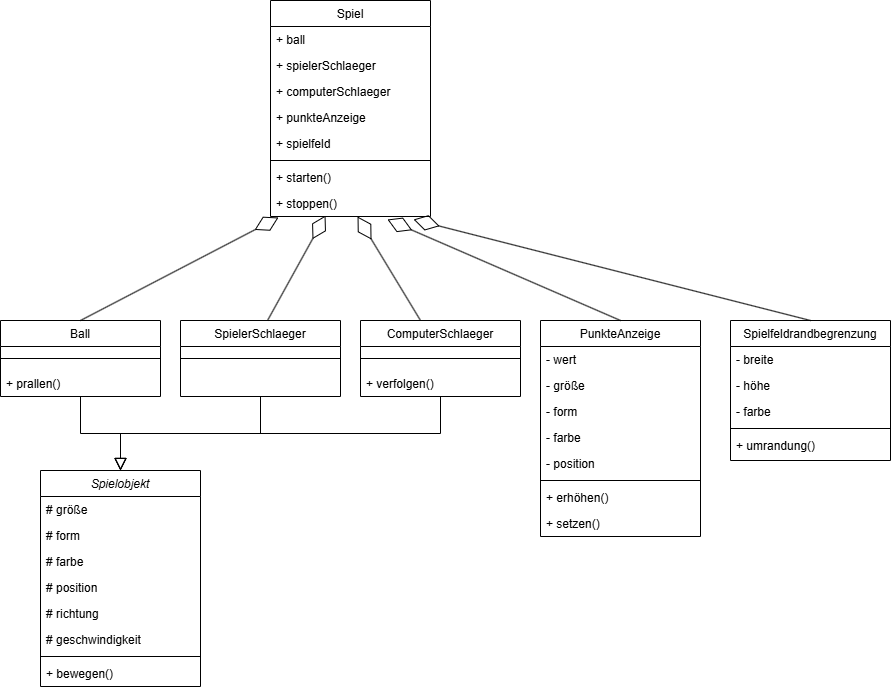
\includegraphics[width=0.7\textwidth]{./img/Konzeptklassendiagramm.png}
    \caption{Konzeptklassendiagramm}
    \label{fig:konzeptklassendiagramm}
\end{figure}
Das Konzeptdiagramm geht nur in Relationen der Klassen und Objekte ein. Sie zeigt die Struktur und Beziehungen zwischen den verschiedenen Klassen darstellt.
\textbf{Zusammenhang der einzelnen Elemente:}
\begin{multicols}{2}
\begin{itemize}[label={},leftmargin=*,noitemsep,topsep=0pt,parsep=0pt]
    \item \textbf{Spiel:} \\
    Die Hauptklasse, die das gesamte Spiel steuert und die anderen Objekte verwaltet. Sie hält die Kontrolle über die Spielobjekte wie Ball, Schläger und Punkteanzeige.
    \item \textbf{SpielObjekt:} \\
    Eine abstrakte Klasse, von der andere Klassen wie Ball, SpielerSchläger und ComputerSchläger erben. Stellt gemeinsame Eigenschaften und Methoden bereit, z. B. Position oder Bewegung.
    \item \textbf{Ball:} \\
    Unterklasse von SpielObjekt, die die Logik und das Verhalten des Balls \textit{(z. B. Bewegung und Kollision)} definiert.
\end{itemize}
\columnbreak
\begin{itemize}[label={},leftmargin=*,noitemsep,topsep=0pt,parsep=0pt]
    \item \textbf{SpielerSchläger und ComputerSchläger:} \\
    Beide erben von SpielObjekt.
    \item \textbf{SpielerSchläger:} \\
    Steuerung durch den Spieler.
    \item \textbf{ComputerSchläger:} \\
    KI-gesteuert.
    \item \textbf{PunkteAnzeige:} \\
    Eine eigenständige Klasse zur Anzeige des aktuellen Punktestands. Sie wird vom Spiel aktualisiert.
    \item \textbf{Spielfeldrandbegrenzung:} \\
    Dient zur Festlegung der Spielfeldgrenzen und Kollisionserkennung \textit{(z. B. Ball prallt ab)}.
\end{itemize}
\end{multicols}
\vspace{-0.9\baselineskip}
\begin{itemize}[label={},leftmargin=*,noitemsep,topsep=0pt,parsep=0pt]
    \item \textbf{Beziehungen:} \\
    Die Klassen, die von SpielObjekt erben, teilen Grundfunktionen wie Position und Bewegung. Die Klasse Spiel hält die Übersicht und sorgt dafür, dass die Spielmechanik \textit{(Bewegung, Kollisionen, Punktestand)} funktioniert.
\end{itemize}
Das Diagramm visualisiert also die Modularität und die Logiktrennung im Pong-Spiel.
\clearpage
\subsection{Implementierungsklassendiagramm}
\begin{figure}[H]
    \centering
    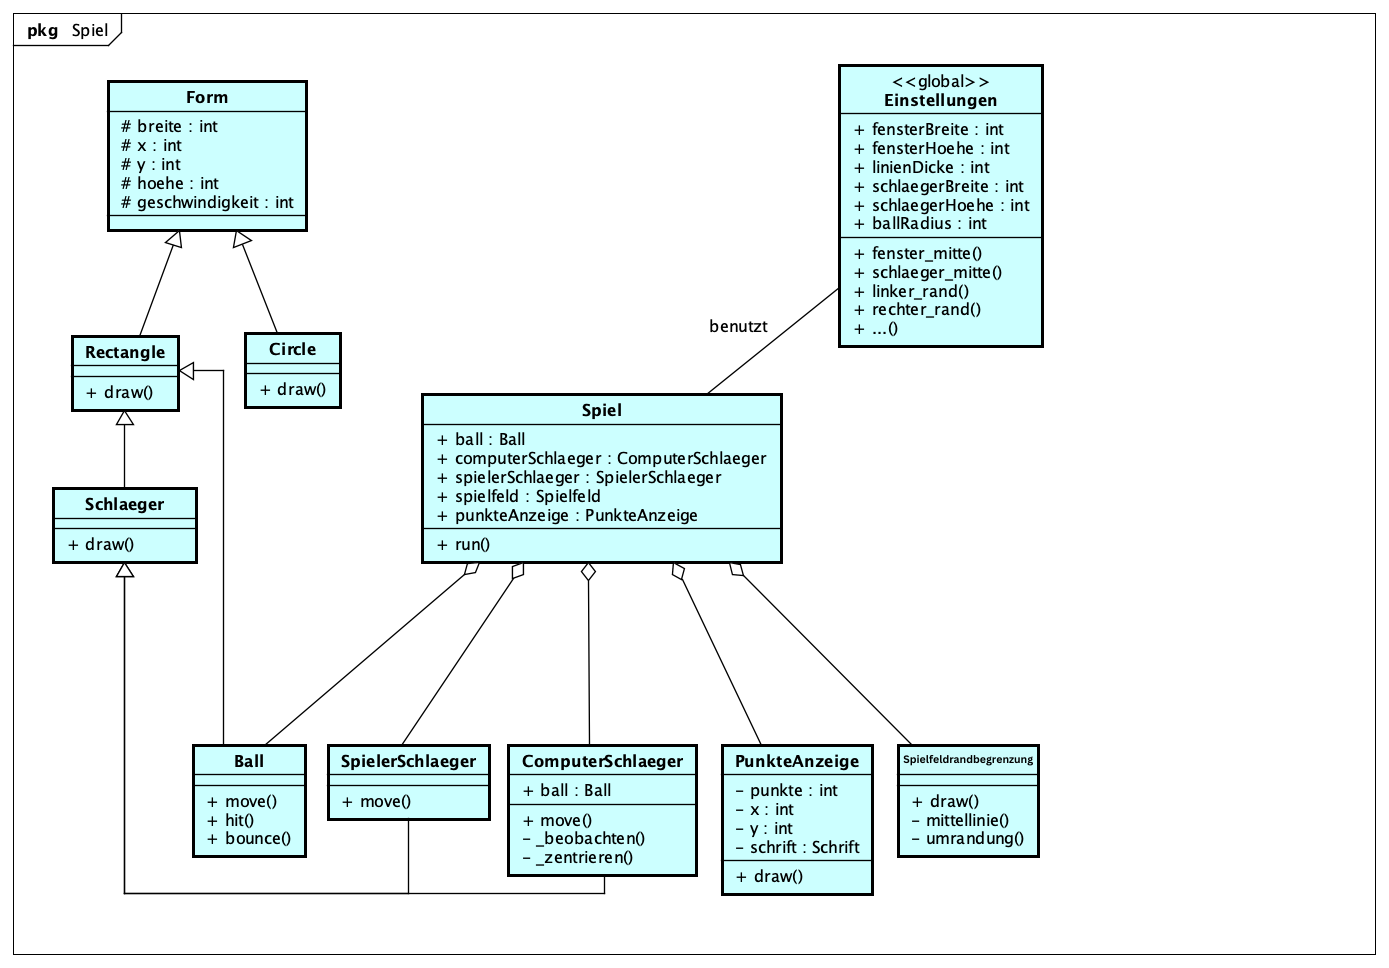
\includegraphics[width=0.7\textwidth]{./img/Implementierungsklassendiagramm.png}
    \caption{Implementierungsklassendiagramm}
    \label{fig:implementierungsklassendiagramm}
\end{figure}
Dieser Entwurf erweitert das vorherige Klassendiagramm und enthält zusätzliche Details sowie einige neue Klassen und Beziehungen. Daher sieht man dieses als eine Erweiterung des Konzeptklassendiagramms an, da dieser alle einzelnen Klassen, in denen Attribute und Methoden festgehalten sind und alle Beziehungen zwischen den Klassen ausführlicher beschreibt. Daher auch der Namen Implementierungsklassendiagramm. Dies ist ein sehr nützliches eigentlich sogar dringend notwendiges Diagramm, da bei der Programmierung ständig darauf zurückgegriffen wird um den Überblick nicht zu verlieren. \par \vspace{\baselineskip} Man kann alle Abhängigkeiten deutlich erkennen. Die Klasse \textbf{Spiel} steht in Relation zu allen Klasse und bildet eine Überklasse. Klar zu erkennen ist, dass die  \textit{\textbf{(globale)} Einstellung} nur eine Abhängigkeit zum Spiel hat und somit ein eigenes unabhängiges Glied zu den anderen Klassen bildet. Die Klassen \textbf{Ball}, \textbf{SpielerSchlaeger}, \textbf{ComputerSchlaeger}, \textbf{PunkteAnzeige} und \textbf{Spielfeld} sind Teile der Klasse \textbf{Spiel}. Wenn man die Klasse \textbf{Form} zurückverfolgt ist zu erkennen, dass die Klassen \textbf{Rectangle} und \textbf{Circle} davon abhängig sind. Die Klasse \textbf{Circle} wird nicht verwendet, jedoch die Klasse \textbf{Rectangle} wird von den Klassen \textbf{Schlaeger} und \textbf{Ball} verwendet. Die Klasse \textbf{Schlaeger} wird wiederum von den Klassen \textbf{SpielerSchlaeger} sowie von der Klasse \textbf{ComputerSchlaeger} beansprucht. Man könnte nun anstatt der Klasse \textbf{Rectangle} die Klasse \textbf{Circle} verwenden und hätte mit einer geringen Änderung komplett andere Darstellung der Objekte. Zu den Klassen sind auch alle Attribute und Methoden sichtbar.
\subsubsection{Zusätzliche Klassen und Beziehungen:}
\vspace{-0.5\baselineskip}
\begin{multicols}{2}
\begin{itemize}[label={},leftmargin=*,noitemsep,topsep=0pt,parsep=0pt]
    \item \textbf{Circle:}
    \begin{itemize}[label={},leftmargin=*,noitemsep,topsep=0pt,parsep=0pt]
        \item Erbt von \textbf{Form} und ist speziell für kreisförmige Objekte wie den Ball gedacht.
    \end{itemize}
\end{itemize}
\columnbreak
\begin{itemize}[label={},leftmargin=*,noitemsep,topsep=0pt,parsep=0pt]
    \item \textbf{Rectangle:}
    \begin{itemize}[label={},leftmargin=*,noitemsep,topsep=0pt,parsep=0pt]
        \item Erbt von \textbf{Form} und implementiert die Methode \textbf{draw()}, um rechteckige Objekte wie zum Beispiel für Schläger darzustellen.
    \end{itemize}
\end{itemize}
\end{multicols}
\clearpage
\begin{itemize}[label={},leftmargin=*,noitemsep,topsep=0pt,parsep=0pt]
    \item \textbf{Form  \textit{(Basisklasse)}:} 
    \begin{itemize}[label={},leftmargin=*,noitemsep,topsep=0pt,parsep=0pt]
        \item Eine abstrakte Klasse, die grundlegende Eigenschaften für grafische Formen definiert, sowie \textbf{breite}, \textbf{höhe}  \textit{(Dimensionen)}, \textbf{X-} und \textbf{Y-Achse}  \textit{(Position auf dem Spielfeld)} und \textbf{geschwindigkeit}  \textit{(Bewegungsgeschwindigkeit)}. Von dieser Klasse erben andere Klassen wie \textbf{Rectangle} und \textbf{Circle}.
    \end{itemize}
    \vspace{0.5\baselineskip}
    \item \textbf{Schläger \textit{(Basisklasse)}:}
    \begin{itemize}[label={},leftmargin=*,noitemsep,topsep=0pt,parsep=0pt]
        \item Eine abstrakte Klasse für alle Schläger, mit der Methode \textbf{draw()} zur Darstellung. Von ihr erben spezifische Schläger:
        \vspace{-0.9\baselineskip}
        \begin{multicols}{2}
        \begin{itemize}[label={},leftmargin=*,noitemsep,topsep=0pt,parsep=0pt]
            \item \textbf{ComputerSchläger:}
            \begin{itemize}[label={},leftmargin=*,noitemsep,topsep=0pt,parsep=0pt]
                \item KI-gestützt, mit internen Methoden wie \textit{\textbf{beobachten()}} und \textit{\textbf{zentrieren()}}.
            \end{itemize}
        \end{itemize}
        \columnbreak
        \begin{itemize}[label={},leftmargin=*,noitemsep,topsep=0pt,parsep=0pt]
            \item \textbf{SpielerSchläger:}
            \begin{itemize}[label={},leftmargin=*,noitemsep,topsep=0pt,parsep=0pt]
                \item Steuerbar durch den Spieler.
            \end{itemize}
        \end{itemize}
        \end{multicols}
    \end{itemize}
    \vspace{-0.4\baselineskip}
    \item \textbf{Einstellungen (global):}
        \begin{itemize}[label={},leftmargin=*,noitemsep,topsep=0pt,parsep=0pt]
            \item Eine Klasse, die globale Konstanten oder Methoden enthält, die für das gesamte Spiel benötigt werden.
            \vspace{-0.9\baselineskip}
            \begin{multicols}{2}
            \begin{itemize}[label={},leftmargin=*,noitemsep,topsep=0pt,parsep=0pt]
                \item \textbf{Attribute:}
                \begin{itemize}[label={},leftmargin=*,noitemsep,topsep=0pt,parsep=0pt]
                    \item Spielfeldmaße \textit{(z.B. \textbf{fensterBreite}, \textbf{fensterHoehe)}}
                    \item Objektgrößen \textit{(z.B. \textbf{schlaegerBreite}, \textbf{ballRadius)}}
                \end{itemize}
            \end{itemize}
            \columnbreak
            \begin{itemize}[label={},leftmargin=*,noitemsep,topsep=0pt,parsep=0pt]
                \item \textbf{Methoden:}
                \begin{itemize}[label={},leftmargin=*,noitemsep,topsep=0pt,parsep=0pt]
                    \item Praktische Helfer wie \textbf{fenster\_mitte()} oder \textbf{linker\_rand()}.
                \end{itemize}
            \end{itemize}
            \end{multicols}
        \end{itemize}
\end{itemize}
\vspace{-0.5\baselineskip}
\subsubsection{Bestehende Klassen mit neuen Details:}
\textbf{Zusätzliche Methoden zu Ball:}
\vspace{-0.9\baselineskip}
\begin{multicols}{3}
\begin{itemize}[label={},leftmargin=*,noitemsep,topsep=0pt,parsep=0pt]
    \item \textbf{move():} Bewegung des Balls.
    \columnbreak
    \item \textbf{hit():} Prüfen, ob der Ball einen Schläger trifft.
    \columnbreak 
    \item \textbf{bounce():} Umsetzung von Abprall-Logik.
\end{itemize}
\end{multicols}
\vspace{-0.9\baselineskip}
\noindent
\textbf{Spiel:} \\ Zentralisiert weiterhin die Steuerung, aber mit einer klareren Darstellung der enthaltenen Objekte \textbf{ball}, \textbf{computerSchläger}, \textbf{spielerSchläger}, \textbf{spielfeld}, \textbf{punkteAnzeige}. Enthält die Methode \textbf{run()}, um das Spiel auszuführen.
\noindent
\textbf{PunkteAnzeige:} Zuständig für die visuelle Darstellung des Punktestands. Verwendet Attribute wie \textbf{punkte} und \textbf{schrift}.
\noindent
\textbf{Spielfeld:} \\ Verantwortlich für die Spielfeld-Darstellung und -Begrenzung mit folgenden Methoden:
\vspace{-0.9\baselineskip}
\begin{multicols}{2}
\begin{itemize}[label={},leftmargin=*,noitemsep,topsep=0pt,parsep=0pt]
    \item \textbf{mittellinie():} Zeichnet die Mittellinie.
    \columnbreak
    \item \textbf{umrandung():} Zeichnet die Spielfeldbegrenzung.
\end{itemize}
\end{multicols}
Die Vererbung erfolgt in der Basisklasse \textbf{Form} für grafische Objekte \textit{(z. B. \textbf{Ball}, \textbf{Schläger})}. \textbf{Schläger} dient als abstrakte Oberklasse für \textbf{Spieler-} und \textbf{Computerschläger}. Dabei steuert und verwendet die Klasse \textbf{Spiel} alle anderen Klassen. \textbf{Einstellungen} liefert globale Konstanten, die von allen Klassen genutzt werden.
\subsubsection{Zweck der Erweiterung:}
\begin{multicols}{2}
\begin{itemize}[label={},leftmargin=*,noitemsep,topsep=0pt,parsep=0pt]
    \item \textbf{Zentralisierung von Einstellungen:} \\ Die Klasse \textbf{Einstellungen} sorgt dafür, dass alle Konstanten und globalen Hilfsmethoden zentral verfügbar sind.
    \columnbreak
    \item \textbf{Wiederverwendbarkeit:} \\ Gemeinsame Eigenschaften \textit{(wie Bewegung oder Zeichnen)} werden in Basisklassen definiert, um Redundanz zu vermeiden.
\end{itemize}
\end{multicols}
\noindent
\textbf{Modularisierung:} \\ Die Trennung in abstrakte Klassen \textit{(z. B. \textbf{Form}, \textbf{Schläger})} und spezialisierte Klassen \textit{(wie \textbf{Ball}, \textbf{SpielerSchläger})} macht den Code flexibler und leichter erweiterbar. \par \vspace\baselineskip
Dieses Diagramm bietet eine klar strukturierte Architektur für das Pong-Spiel und erleichtert sowohl die Entwicklung als auch spätere Änderungen oder Erweiterungen.
\clearpage
% ======================== Implementierung ========================
\section{Implementierung}
Das Spiel läuft auf einem Raspberry Pi läuft über eine Appliance, wobei wird Python und die Py Game-Bibliothek verwendet und alle relevanten Klassen, Objekte und Spiellogik sind in separaten Python-Dateien Spiel organisiert untergebracht. \par \vspace\baselineskip
Das Projekt wurde in mehrere Module unterteilt, um die Wartbarkeit und Erweiterbarkeit des Codes zu verbessern. Der Hauptkomponent des Spiels ist dabei das Spielbibliothek \textit{(\textbf{spiel.py})}, welches alle Spielklassen und -objekte enthalten. Darauf wird dann zugegriffen um ganz sauber im Code nur die Regeln, die Interaktion der Spielobjekte und die Steuerung zu definieren. Dies erfolgt mittels Erdungen und übernehmen der Klassen beziehungsweise Objekte. \par \vspace\baselineskip
Py Game wird als Grafikbibliothek genutzt, um die verschiedenen Spielobjekte zu visualisieren und mit Benutzeraktionen zu interagieren. Die Funktionen von Py Game wie \textbf{rect()} und \textbf{circle()} ermöglichen das Zeichnen von Rechtecken \textit{(\textbf{Schläger})} und Kreisen \textit{(\textbf{Ball})}. \par \vspace\baselineskip
Auf dem Raspberry Pi wurde das Spiel so optimiert, dass es auf der limitierten Hardware läuft. Daher auch bei \textit{(8) Test} der Fehler mit dem Computerschläger. Der Raspberry Pi stellt dabei die Plattform dar, auf der das Spiel gestartet und ausgeführt wird, und das Py Game-Rendering wird direkt auf dem angeschlossenen Bildschirm dargestellt. \par \vspace\baselineskip
Das Projekt verwendet eine objektorientierte Struktur, wobei jede Spielfunktionalität in Klassen gekapselt ist. Die Py Game-Bibliothek wird verwendet, um das Spiel visuell darzustellen und die Benutzerinteraktion zu ermöglichen. Der Raspberry Pi dient dabei als Hardware-Plattform für das Spiel.
\clearpage
% ======================== Test ========================
\section{Test}
Eine Testphase ist essentiell, um eine letzte Kontrolle zu haben, ob alle Ziele tatsächlich auch erreicht worden sind, Fehler im Spiel zu finden und diese zu beheben, die Benutzererfahrung zu verbessern und sicherzustellen, dass alle Funktionen wie gewünscht funktionieren. Sie hilft auch, mögliche technische Probleme zu identifizieren und die Spielbalance zu überprüfen, bevor das Spiel veröffentlicht wird beziehungsweise dem Kunden übergeben wird. \par \vspace\baselineskip
\textbf{Dies sind die Mangeln die noch hätten behoben müssen:}
\begin{itemize}[noitemsep,topsep=0pt,parsep=0pt,partopsep=0pt]
    \item Der Start Button fehlt.
    \item Der Computerschläger folgt nicht durchgängig dem Ball. Sobald der Ball die Mitter des Spielfeldes überschreitet beim entfernen positioniert sich der Computerschläger mittig.
    \item Der Ball kann hinter dem Spielerschläger gefangen werden, wenn der Ball von hinten den Spielerschläger berührt erhält man in fünferschritten Punkte.
\end{itemize}
% ======================== Übergabe / Projektabschluss ========================
\section{Übergabe / Projektabschluss}
Bei einem normalen Projekt müsste man die Übergabe in folgenden Schritten bearbeitet abschließen: \par \vspace\baselineskip
\begin{itemize}[noitemsep,topsep=0pt,parsep=0pt,partopsep=0pt]
    \item Übergabe und Einführung vor Ort beim Kunden
    \item Handbuch
    \item Schulung
    \item Ansprechpartner für Probleme benennen
    \item Abschlussarbeit mit allen Projektpartnern
\end{itemize}
\vspace\baselineskip
In diesem Fall erfolgt dieser mit der Absendung der B-Aufgabe.
\clearpage
% ======================== Schlussfolgerung und eigene Reflexion ========================
\section{Schlussfolgerung und eigene Reflexion}
Im Großen und Ganzen ist das Projekt „\textbf{Pong}“ ein relativ einfach zu verstehendes Einsteigerprojekt. Dass viele Aufgaben nicht erledigt werden mussten, die andernfalls viel Zeit und Aufwand gekostet hätten, hat das Verständnis für die wesentlichen Aspekte des Projekts erleichtert. Dadurch konnten wir uns gezielt auf die Kernaufgaben konzentrieren. Zudem hatten wir jederzeit die Möglichkeit, den Projektbetreuer zu kontaktieren und seine Hilfe in Anspruch zu nehmen, was uns das Gefühl gab, nicht im Stich gelassen zu werden. Dies war eine wichtige Motivation, das Projekt bis zum Ende durchzuziehen. \par \vspace\baselineskip
Was ich persönlich ebenfalls als erfolgreich empfunden habe, war, dass wir zu Beginn in einer Gruppe gearbeitet haben, mit vielen Diskussionen und gemeinschaftlichen Aufgaben. Erst später mussten wir uns dann mit den kleineren Details eigenständig befassen. Das bedeutete, dass wir nicht von Anfang an mit voller Belastung konfrontiert wurden. \par \vspace\baselineskip
Die Balance zwischen dem theoretischen und dem praktischen Teil war meiner Meinung nach ziemlich ausgewogen. Man musste weder wegen einer endlosen, ermüdenden Theorievorlesung einschlafen \textit{(Theorieteil)}, noch fehlten einem wichtige Informationen, die das Verständnis des Praxisteils erschwert hätten. \par \vspace\baselineskip
Jedoch denke ich, dass dieses Projekt für Personen ohne Programmierkenntnisse oder ein ausgeprägtes IT-Verständnis etwas anspruchsvoller gewesen sein könnte. Besonders, weil man zum ersten Mal programmierte und zwei Bibliotheken einbinden musste, ohne genau zu wissen, was diese Bibliotheken sind, welche Rolle sie spielen und möglicherweise auch nicht alles auf Anhieb verstanden hat. Dies hat sicherlich mehr Fragen aufgeworfen, als man sich zu stellen traute. Zwar war der Hauptcode verständlich, doch blieben die Bibliotheken ein gewisses Fragezeichen. Ich denke, die Intention hinter den Aufgaben 2-4 war, dass man sich eigenständig mit der „\textbf{spiel.py}“-Bibliothek auseinandersetzt, und falls man Hilfe benötigt, hätte man diese jederzeit einholen können. Mit dieser Herangehensweise ist es durchaus nachvollziehbar. Abgesehen davon würde ich das Projekt möglicherweise genauso vorbereit. \par \vspace\baselineskip
Ein weiterer in meinen Augen, doch einer der wichtigsten Vorteile mit einem Projekt mit Bibliotheken zu starten ist, dass auch, wenn man sich denken könnte, „\textit{Als erstes Projekt gleich so ein etwas anspruchsvolleres Projekt? Wie soll ich das mur schaffen?}“ ist, dass man am Ende sagen kann: „\textit{Ich habe gerade erst mit Python programmieren angefangen und tatsächlich bereits ein Spiel programmiert. Ich kann es also doch schaffen!}“. \par \vspace\baselineskip
Motiviert zu sein und motiviert zu bleiben entscheidet am Ende, ob man etwas schafft oder doch scheitert. Denn, man hat immer die Möglichkeit sich weiter zu entwickeln und fehlende Lücken, fehlendes Wissen oder fehlendes können anzueignen. Man muss sich nur in Bewegung setzten und dies funktioniert bei den meisten Menschen Großteils durch Motivation. \par \vspace\baselineskip
Daher möchte ich mich an den Dozenten bedanken.
\clearpage
% ======================== Aufgabe 2 (Farbige Objekte) ========================
\section{Aufgabe 2 \textit{(Farbige Objekte)}}
\subsection{Geänderter Quellcode}
\begin{lstlisting}[language=Python, captionpos=b, caption={Aufgabe 2: Geänderter Quellcode}, label=lst:aufgabe-2-geaenderter-quellcode]
class ColoredBall(Ball):
    def __init__(self, x, y, breite, hoehe, geschwindigkeit, farbe):
        super().__init__(x, y, breite, hoehe, geschwindigkeit, farbe)
        self.farbe = farbe
\end{lstlisting}
\par \vspace\baselineskip
Es wurde eine Klasse erstellt \textbf{ColoredBall(Ball)} der die Eigenschaften der Klasse Ball erbt, daher steht dieses in Klammer. Es werden alle Eigenschaften über den Konstruktor der Superklasse \textbf{super()}. initialisiert und mit \textbf{self.farbe = farbe} als \textit{\textbf{farbe}} umdefiniert. \par \vspace\baselineskip
\begin{lstlisting}[language=Python, captionpos=b, caption={Aufgabe 2: farbe}, label=lst:aufgabe-2-farbe]
farbe = pygame.Color(255, 0, 0, 0)
\end{lstlisting}
\par \vspace\baselineskip
In \textbf{ball = ColoredBall} unter \textbf{def main()} wurde es mit \textit{\textbf{farbe}} erweitert und mittels der Pygame Bibliothek und rgba Farbencode die Farbe Rot verliehen. \par \vspace\baselineskip
\textbf{rgba:}
\begin{itemize}[noitemsep,topsep=0pt,parsep=0pt]
    \item \textbf{r (int)} – Rotwert im Bereich von 0 bis 255
    \item \textbf{g (int)} – Grünwert im Bereich von 0 bis 255
    \item \textbf{b (int)} – Blauwert im Bereich von 0 bis 255
    \item \textbf{a (int)} – Alphawert \textit{(für die Transparenz)} im Bereich von 0 bis 255
\end{itemize}
\par \vspace\baselineskip
Die Farben der Schläger wurden direkt verändert. Ohne eine weitere Klasse zu definieren. Somit wurden alle zwei Optionen eingesetzt. \par \vspace\baselineskip
\begin{lstlisting}[language=Python, captionpos=b, caption={Aufgabe 2: spielerSchlaeger}, label=lst:aufgabe-2-spielerschlaeger]
farbe = 'green'
\end{lstlisting}
\par \vspace\baselineskip
In \textbf{spielerSchlaeger = Schlaeger} wurde das ursprünglich in \textit{\textbf{spiele.py}} vor definierte \textbf{farbe=pygame.Color('white')} mit \textbf{farbe = 'green'} ersetzt.  \par \vspace\baselineskip
\begin{lstlisting}[language=Python, captionpos=b, caption={Aufgabe 2: computerSchlaeger}, label=lst:aufgabe-2-computerschlaeger]
farbe = 'blue'
\end{lstlisting}
\par \vspace\baselineskip
Und in \textbf{computerSchlaeger = AutoSchlaeger} wurde wiederum das ursprünglich in \textit{\textbf{spiele.py}} vor definierte \textbf{farbe=pygame.Color('white')} mit \textbf{farbe = 'blue'} ersetzt.
\clearpage
\subsection{Konzeptklassendiagramm}
\begin{figure}[H]
    \centering
    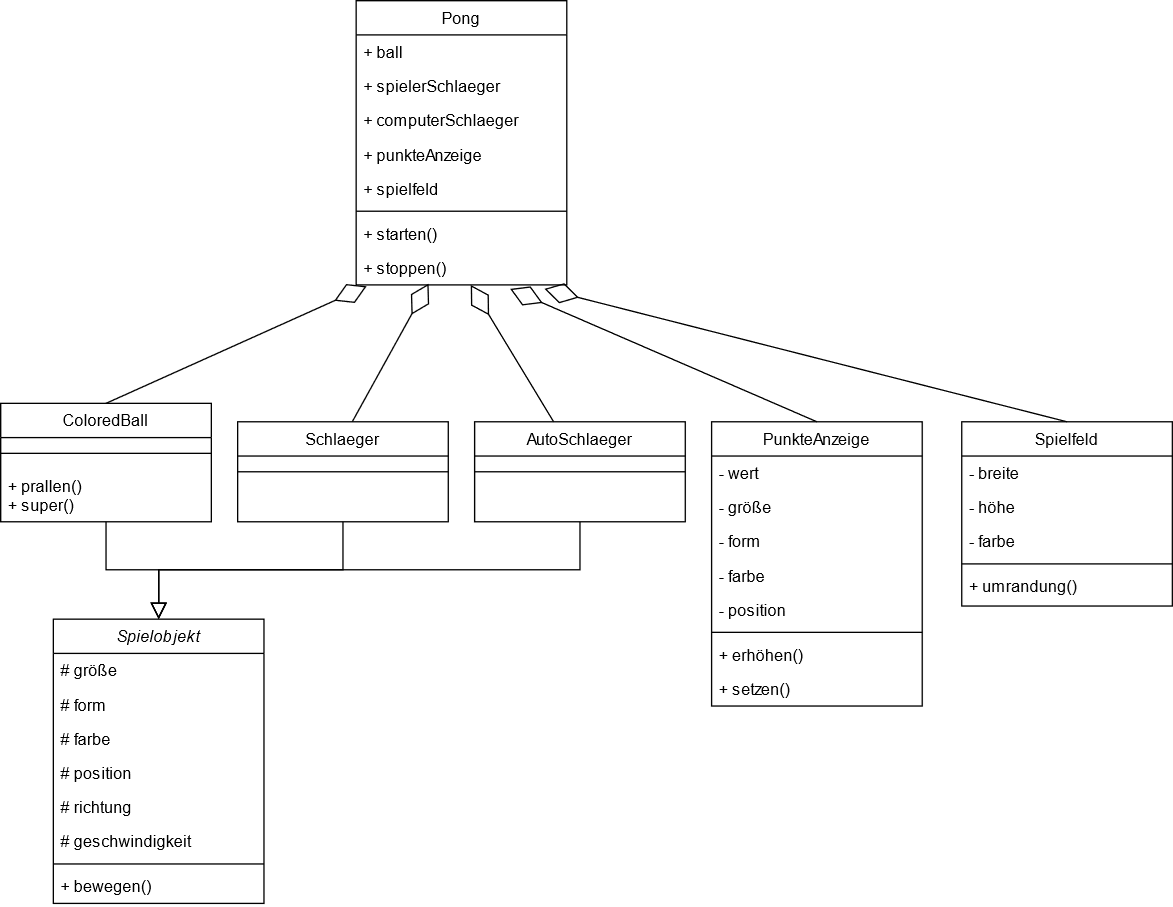
\includegraphics[width=0.8\textwidth]{./img/Aufgabe2Konzeptklassendiagramm.png}
    \caption{Aufgabe 2: Konzeptklassendiagramm}
    \label{fig:aufgabe2konzeptklassendiagramm}
\end{figure}
\subsection{Ergebnis}
\begin{figure}[H]
    \centering
    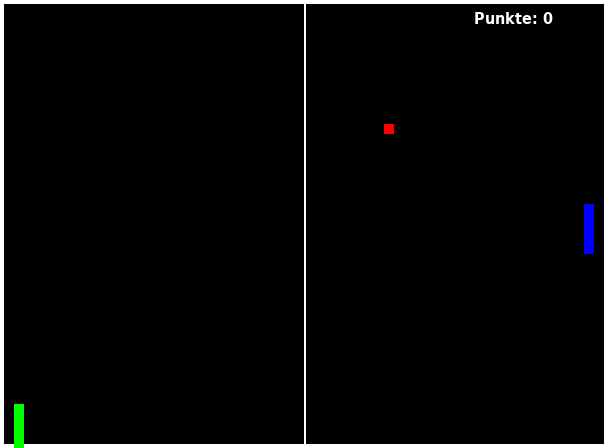
\includegraphics[width=0.8\textwidth]{./img/Aufgabe2Ergebnis.png}
    \caption{Aufgabe 2: Ergebnis}
    \label{fig:aufgabe2ergebnis}
\end{figure}
\clearpage
% ======================== Aufgabe 3 (Tastatursteuerung) ========================
\section{Aufgabe 3 \textit{(Tastatursteuerung)}}
\subsection{Geänderter Quellcode}
\begin{lstlisting}[language=Python, captionpos=b, caption={Aufgabe 3: TastaturSchlaeger(Schlaeger)}, label=lst:aufgabe-3-tastaturschlaeger-schlaeger]
class TastaturSchlaeger(Schlaeger):
    def movekey(self, pos):
        self.rect.y = self.rect.y + (pos * self.geschwindigkeit)
\end{lstlisting}
\par \vspace\baselineskip
Eine weitere Klasse wurde erstellt \textbf{TastaturSchlaeger(Schlaeger)} der die Instanzen von Schlaeger erbt um der Maussteuerung zusätzlich eine Tastatursteuerung hinzuzufügen. Dafür wird eine Funktion \textbf{movekey(self, pos)} definiert der die Position \textit{(\textbf{pos})} und die Geschwindigkeit \textit{(\textbf{geschwindigkeit})} angibt. \par \vspace\baselineskip
\begin{lstlisting}[language=Python, captionpos=b, caption={Aufgabe 3: SpielErweitert(Spiel)}, label=lst:aufgabe-3-spielerweitert-Spiel]
class SpielErweitert(Spiel):
    def _behandle(self, event):
        event = super()._behandle(event)
        if not event:
            return
        if event.type == pygame.KEYDOWN:
            self._reagiere_auf_tastatur(event)
    
    def _reagiere_auf_tastatur(self, event):
        if event.key == pygame.K_UP:
            self._spieler.movekey(-10)
        elif event.key == pygame.K_DOWN:
            self._spieler.movekey(+10)
        elif event.key == pygame.K_ESCAPE:
            pygame.event.post(pygame.event.Event(pygame.QUIT))
\end{lstlisting}
\par \vspace\baselineskip
Zu guter Letzt eine Klasse \textbf{SpielErweitert(Spiel)} der von Spiel erbt und mittels 2 Funktionen \textbf{\_behandle(self, event)} und \textbf{\_reagiere\_auf\_tastatur(self, event)} den Workflow der Tastatursteuerung definiert. \par \vspace\baselineskip
\begin{lstlisting}[language=Python, captionpos=b, caption={Aufgabe 3: \_behandle(self,event)}, label=lst:aufgabe-3-behandle-self-event]
def _behandle(self, event):
    event = super()._behandle(event)
\end{lstlisting}
\par \vspace\baselineskip
Bei der ersten Funktion \textbf{\_behandle(self, event)} werden zuerst die Eigenschaften für das Schließen sowie die Maussteuerung mittels den Konstruktor der Superklasse \textbf{super()}. initialisiert und als \textit{\textbf{event}} definiert.
\clearpage
\begin{lstlisting}[language=Python, captionpos=b, caption={Aufgabe 3: Event-Handling}, label=lst:aufgabe-3-event-handling]
if not event:
    return
\end{lstlisting}
\par \vspace\baselineskip
Wenn nichts zurückkommt, dann Funktion zurückzukehren \textit{(die Funktion wurde behandelt)}. \par \vspace\baselineskip
\begin{lstlisting}[language=Python, captionpos=b, caption={Aufgabe 3: KEYDOWN Prüfung}, label=lst:aufgabe-3-keydown-pruefung]
if event.type == pygame.KEYDOWN:
    self._reagiere_auf_tastatur(event)
\end{lstlisting}
\par \vspace\baselineskip
Wenn die \textbf{$\uparrow$ Taste} \textit{(\textbf{Keydown})} betätigt wird, wird darauf reagiert. Sprich es wird überprüft, ob die Taste betätigt wird. \par \vspace\baselineskip
\begin{lstlisting}[language=Python, captionpos=b, caption={Aufgabe 3: \_reagiere\_auf\_tastatur(self,event)}, label=lst:aufgabe-3-reagiere-auf-tastatur-self-event]
def _reagiere_auf_tastatur(self, event):
\end{lstlisting}
\par \vspace\baselineskip
Bei der ersten Funktion haben wir überprüft, ob die Taste betätigt wird. Nun bei der zweiten Funktion, welches zugleich eine Methode ist, wird definiert was danach geschehen soll. \par \vspace\baselineskip
\begin{lstlisting}[language=Python, captionpos=b, caption={Aufgabe 3: Tastensteuerung}, label=lst:aufgabe-3-tastensteuerung]
if event.key == pygame.K_UP:
    self._spieler.movekey(-10)
elif event.key == pygame.K_DOWN:
    self._spieler.movekey(+10)
\end{lstlisting}
\par \vspace\baselineskip
Wenn die \textbf{$\uparrow$ Taste} \textit{(\textbf{Keyup})} betätigt wird, wird der Funktion \textit{(\textbf{movekey}(\textbf{-10}))} -10 Pixel/Pfeiltaste subtrahiert. \par Wenn die \textbf{$\uparrow$ Taste} \textit{(\textbf{Keydown})} betätigt wird, wird der Funktion \textit{(\textbf{movekey}(\textbf{+10}))} +10 Pixel/Pfeiltaste addiert. \par \vspace\baselineskip Dadurch haben wir einen Trigger der eine Aktion durchführt welches dafür sorgt, dass sich der Spielerschläger bewegt. \par \vspace\baselineskip
\noindent
\textbf{Fußnote:} \par
\textit{In dieser Aufgabe gibt es kein Screenshot, da nur eine Tastatursteuerung dazugegeben worden ist und das Bild genau so aussieht wie in Aufgabe 2.}
\clearpage
\subsection{Konzeptklassendiagramm}
\begin{figure}[H]
    \centering
    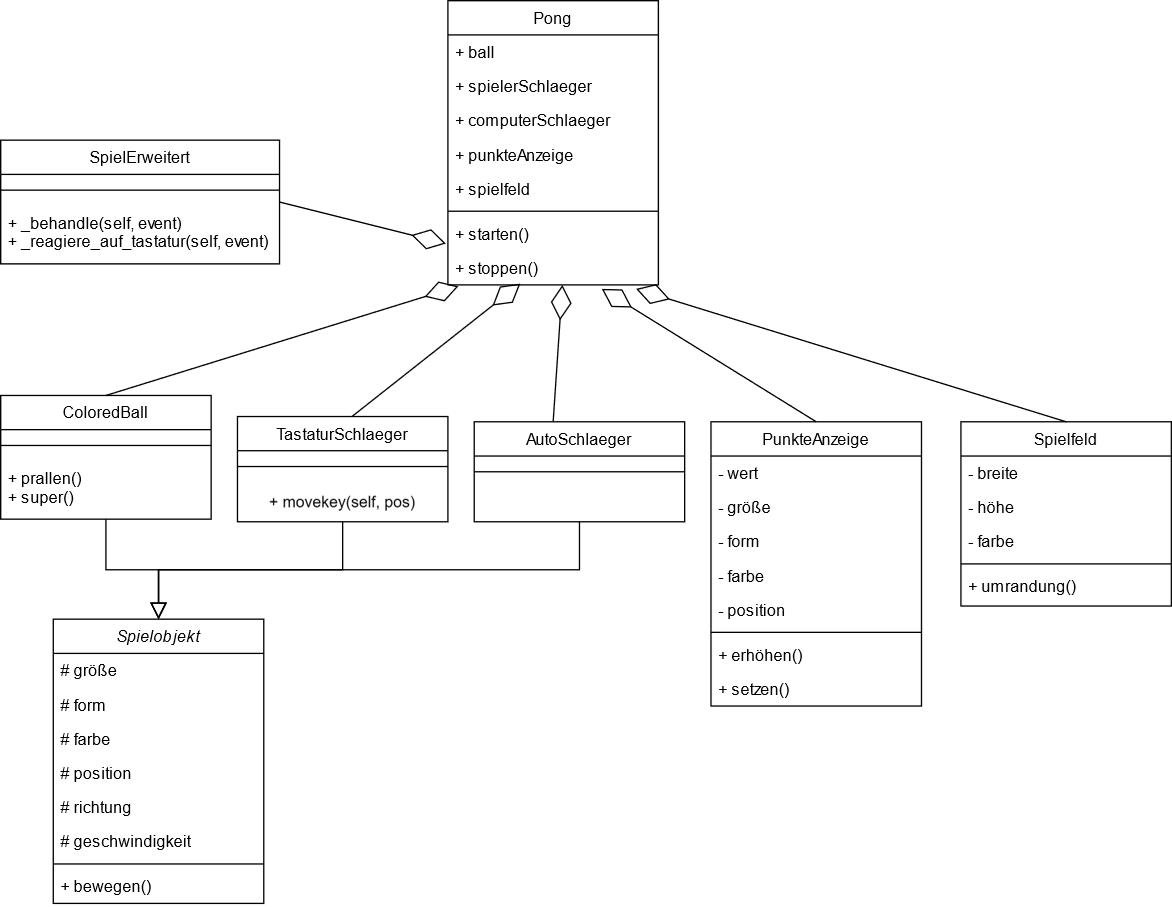
\includegraphics[width=1\textwidth]{./img/Aufgabe3Konzeptklassendiagramm.png}
    \caption{Aufgabe 3: Konzeptklassendiagramm}
    \label{fig:aufgabe3konzeptklassendiagramm}
\end{figure}
\clearpage
% ======================== Aufgabe 4 (Erweiterte Ballfarb-Logik) ========================
\section{Aufgabe 4 \textit{Erweiterung}}
\subsection{Geänderter Quellcode}
\begin{lstlisting}[language=Python, captionpos=b, caption={Aufgabe 4: ColoredBall Klasse mit bounce-Methode}, label=lst:aufgabe-4-coloredball]
class ColoredBall(Ball):
    def __init__(self, x, y, breite, hoehe, geschwindigkeit, farbe):
        super().__init__(x, y, breite, hoehe, geschwindigkeit, farbe)
        self.farbe = farbe
    
    def bounce(self, axis):
        super().bounce(axis)
        if axis == 'x':
            self.farbe = pygame.Color(0, 0, 0, 0)
        elif axis == 'y':
            self.farbe = pygame.Color(255, 0, 0, 0)
\end{lstlisting}
\par \vspace\baselineskip
Als Erweiterung wurde die geerbte Funktion \textbf{bounce(self, axis)} welches für die Richtungsänderung des Balles sorgt unter der Klasse \textbf{Ball(Rectangle)} erweitert, in dem unter der zuvor deklarierten Klasse \textbf{ColoredBall(Ball)} mittels Initialisierung der Eigenschaften über den Konstruktor der Superklasse \textbf{super()} und der Erweiterung. \par \vspace\baselineskip
\begin{lstlisting}[language=Python, captionpos=b, caption={Aufgabe 4: bounce-Methode im Detail}, label=lst:aufgabe-4-bounce]
def bounce(self, axis):
    super().bounce(axis)
    if axis == 'x':
        self.farbe = pygame.Color(0, 0, 0, 0)
    elif axis == 'y':
        self.farbe = pygame.Color(255, 0, 0, 0)
\end{lstlisting}
\par \vspace\baselineskip
Die Funktion wird deklariert und geerbt. Wenn die Achse des Balles der X-Achse entspricht, so wird die Farbe auf schwarz gesetzt. Wenn die Achse des Balles der Y-Achse entspricht, so wird die Farbe auf Rot gesetzt. \par Somit ist eine gewisse Schwierigkeit gegeben, da man bei jedem Kontakt des Balles bis zum nächsten Kontakt der Ball nicht sichtbar ist. \par \vspace\baselineskip
\clearpage
\subsection{Konzeptklassendiagramm}
\begin{figure}[H]
    \centering
    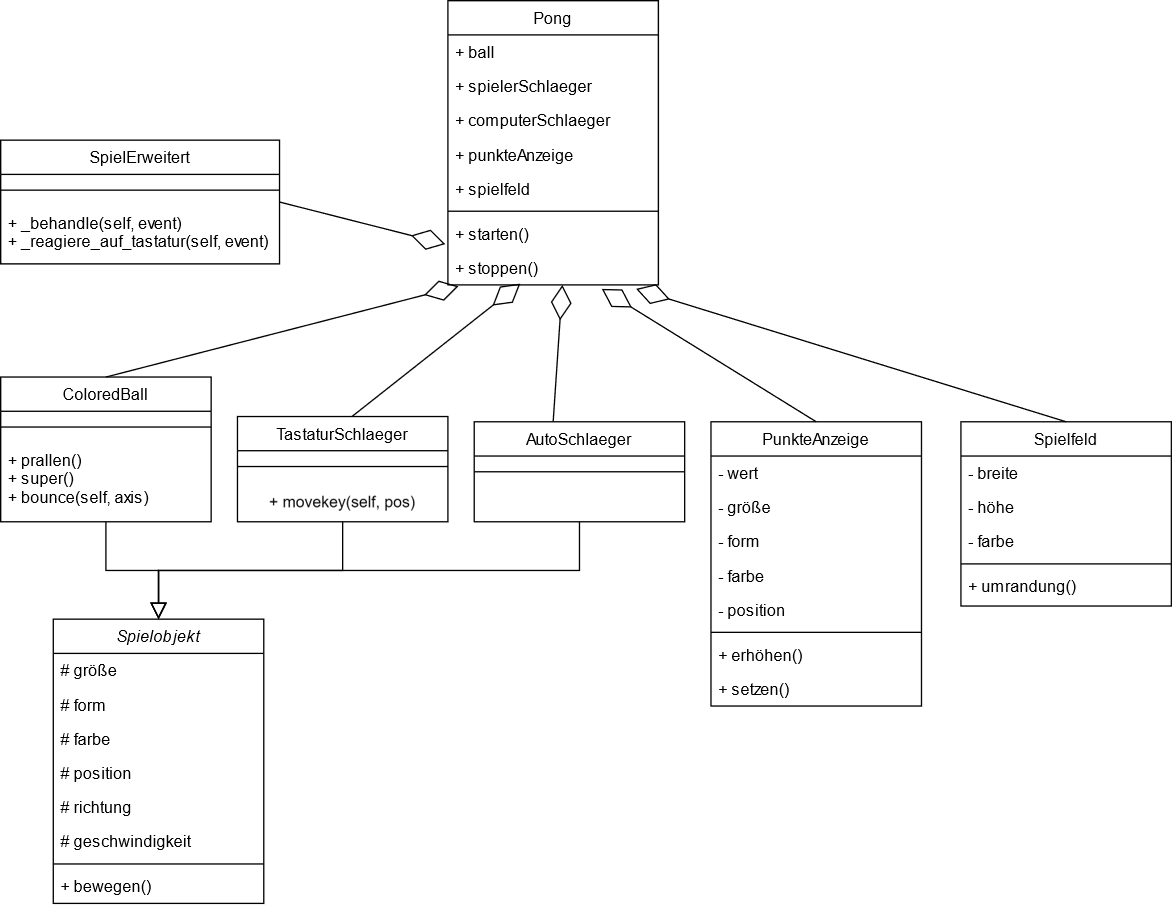
\includegraphics[width=1\textwidth]{./img/Aufgabe4Konzeptklassendiagramm.png}
    \caption{Aufgabe 4: Konzeptklassendiagramm}
    \label{fig:aufgabe4konzeptklassendiagramm}
\end{figure}
\clearpage
\subsection{Ergebnis}
Man kann deutlich erkennen, wie sich die Farbe des Balles nach dem Kontakt mit dem blauen Schläger verändert. \par \vspace\baselineskip
\begin{figure}[H]
    \centering
    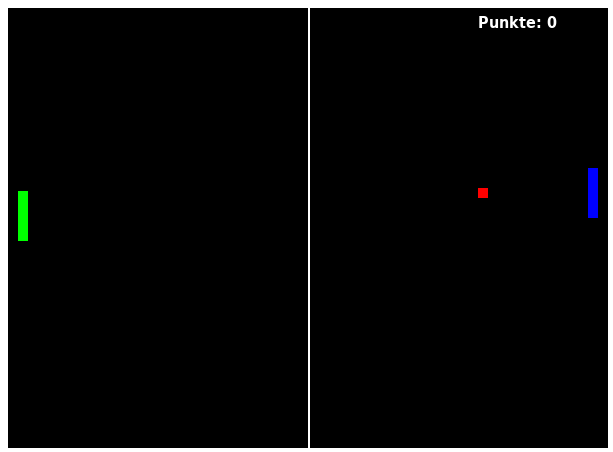
\includegraphics[width=0.8\textwidth]{./img/Aufgabe4Ergebnis.png}
    \caption{Aufgabe 4: Ergebnis}
    \label{fig:aufgabe4ergebnis}
\end{figure}
\begin{figure}[H]
    \centering
    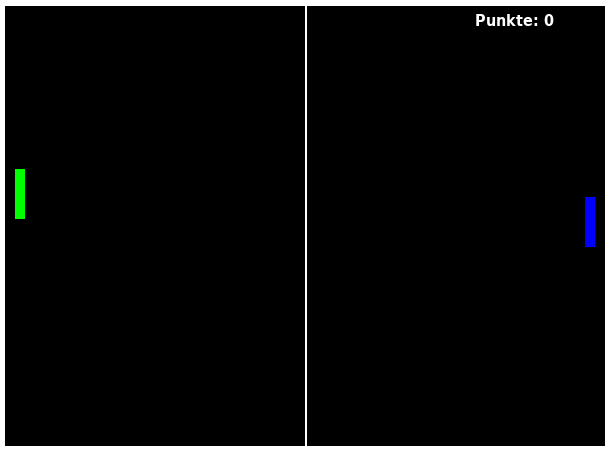
\includegraphics[width=0.8\textwidth]{./img/Aufgabe4ErgebnisII.png}
    \caption{Aufgabe 4: ErgebnisII}
    \label{fig:aufgabe4ergebnisii}
\end{figure}
\clearpage
% ======================== ChatGPT 4o mini Pomps ========================
\section*{ChatGPT 4o mini Pomps}
\addcontentsline{toc}{section}{ChatGPT 4o mini Pomps}
\begin{itemize}[label={},noitemsep,topsep=0pt,parsep=0pt,partopsep=0pt,leftmargin=*]
    \item \textbf{Implementierungsklassendiagramm} \dotfill
    \begin{itemize}[label={},noitemsep,topsep=0pt,parsep=0pt,partopsep=0pt,leftmargin=*]
        \item Kannst du diesen Entwurf ganz kurz erklären? \dotfill
    \end{itemize}
    \item \textbf{Konzeptklassendiagramm} \dotfill
    \begin{itemize}[label={},noitemsep,topsep=0pt,parsep=0pt,partopsep=0pt,leftmargin=*]
        \item Kannst du ganz kurz diese Erklärung mit den Fehlenden erweitern? \dotfill
    \end{itemize}
\end{itemize}
\end{document}